\documentclass[8pt, A4]{article}

%Margenes de la pagina.  otra opcion, usar \usepackage{a4wide}
\usepackage[paper=a4paper, left=0.8cm, right=0.8cm, bottom=1.3cm, top=0.9cm]{geometry}
\usepackage{color}

%este paquete permite incluir acentos.  Notar que espera un formato ANSI-blah de archivo.  Si en lugar de eso se tiene un utf8 (usual en los linux), entonces usar \usepackage[utf8]{inputenc}
\usepackage[utf8]{inputenc}

%Este paquete es para que algunos titulos (como Tabla de Contenidos) esten en castellano
\usepackage[spanish]{babel}

%El siguiente paquete permite escribir la caratula facilmente
\usepackage{caratula}

\usepackage{aed2-symb,aed2-itef,aed2-tad,aed2-tokenizer,modulos_diseno, ./algorithms/clrscode3e}
\usepackage{framed}
\usepackage{amsmath}

\usepackage{graphicx}

%Datos para la caratula
\materia{Sistemas Operativos}

\titulo{Trabajo Pr\'actico 1 - Cachalotes}


\integrante{Ortiz de Zarate, Juan Manuel}{403/10}{jmanuoz@gmail.com}
\integrante{Kujawski, Kevin}{459/10}{kevinkuja@gmail.com}
\integrante{Carreiro, Martin}{45/10}{carreiromartin@gmail.com}

\begin{document}
%numero de grupo
%{\hfill\Huge 10}
%esto construye la caractula
\maketitle 

 
 \tableofcontents

 \newpage

\section{Ejercicio 2}

%SI QUIEREN AGREGAR IMAGENES COPIEN EL SIGUIENTE CODIGO
%\begin {center}
%\includegraphics[width=12cm]{./graphEj1.jpg}
% grafico.eps: 0x0 pixel, 300dpi, 0.00x0.00 cm, bb=50 50 410 302
%\end {center}

  \newpage
\section{Ejercicio 4}

%SI QUIEREN AGREGAR IMAGENES COPIEN EL SIGUIENTE CODIGO
%\begin {center}
%\includegraphics[width=12cm]{./graphEj1.jpg}
% grafico.eps: 0x0 pixel, 300dpi, 0.00x0.00 cm, bb=50 50 410 302
%\end {center}


En el siguiente gráfico se puede observar el diagrama de Gantt para el lote LoteEj4.tsk ejecutadas mediante el scheduler Round-Robin con un quantum igual 11.

\begin {center}
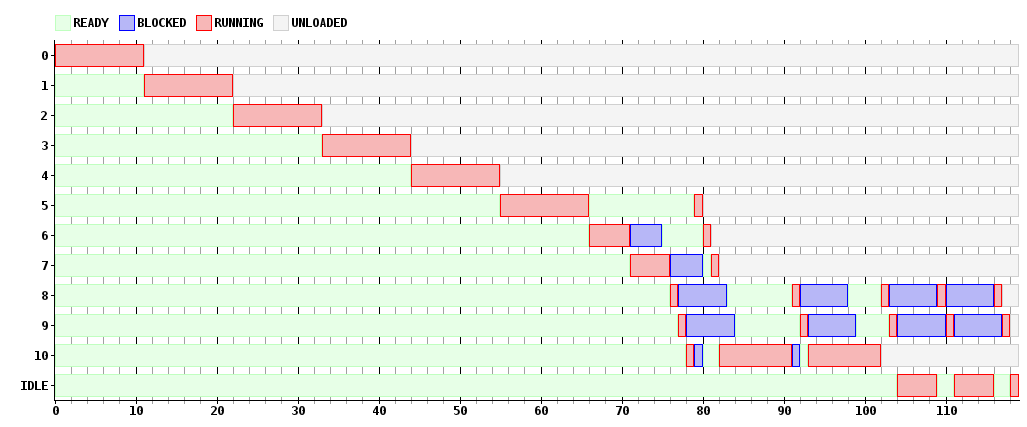
\includegraphics[width=16cm]{../simusched/outputs/outEj4.png}
\end {center}

Descripción del diagrama:
En la ejecución de las primeras 5 tareas se parece al scheduler FIFO, debido a que puede ejecutarlas enteras en 1 solo Quantum. Pero a partir de la quinta tarea podemos observar el funcionamiento del Round-Robin en todo su esplendor.
La tarea número 5 se ejecuta durante 11 ciclos y antes de ser finalizada el scheduler la saca y pone a la siguiente debido a que se termino su 'tiempo' (llego a los 11 ciclos, es decir alcanzo el quantum).
La tarea número 6 se ejecuta durante 4 ciclos y luego se bloquea durante otros 4 utlizando un ciclo extra para la ejecución de la llamada. Cuando esta tarea procede a bloquearse el scheduler (a diferencia del FIFO) cambia a la tarea siguiente y esta procede de la misma manera.
Las 2 tareas siguientes se comportan muy parecido nada mas que lo primero que hacen es bloquearse y por lo tanto el scheduler las deja solo 1 ciclo en ejecucion.
Por último la tarea 10 también realiza un bloqueo apenas se ejecuta por una cuestion aleatoria (la tarea 10 es la taskBatch y el momento en que ejecuta el bloqueo es aleatorio).
Luego de haber ejecutado lo correspondiente a todas las tareas vuelve a la número 5 (que no había sido terminada de ejecutar), una vez que ésta termina, cambia a la siguiente (aunque no se haya cumplido el quantum, si no desperdiciaria ciclos de las tareas que ya se encuentran en estado 'ready'). Lo mismo sucede con las dos tareas siguientes.
Como la tarea número 8 sigue bloqueada, no la ejecuta al igual que la tarea 9.
Carga la tarea 10 hasta que esta se vuelve a bloquear y la cambia por la tarea 8 (que ya no se encuentra bloqueada) ésta se bloquea y repite el procedimiento para la tarea 9. 
Termina de ejecutar la tarea 10 y acá podemos observar que hay un momento en que si bien las tareas 8 y 9 son las únicas tareas cargadas no finalizadas aún no las carga debido a que se encuentran bloqueadas y por eso se corre la tarea IDLE hasta que se desbloquea alguna de las 2.
Finalmente repite esa ultima secuencia 1 vez mas y finaliza la ejecución de todas las tareas.

Resumen:
A diferencia del FIFO este scheduler no (necesariamente) ejecuta una tarea hasta que esta finalize, sino que hasta que se cumpla el Quantum de ciclos, el proceso se bloquee o efectivamente concluya. Por otro lado también cabe enfatizar que el orden en que las alterna esta dado por una cola en la que las tareas se encuentran ordenandas por orden llegada, donde una vez ejecutada la última vuelve a la primera no acabada y sólo ejecuta la tarea idle en caso que el resto de las tareas se encuentren bloqueadas.
Finalmente este scheduler es mejor (en comparación al FIFO) cuando se desea dar la sensación de que se está ejecutando todo en simultáneo (multiprogramación), obviamente con un rango de quantum tal que sea imperceptible para el usuario y hace un mejor uso del cpu ya que cuando una tarea se encuentra bloqueada la quita y pone a otra tarea que esté en estado READY para no desperdiciar ciclos de ejecución.

  \newpage
 \section{Ejercicio 7}

%SI QUIEREN AGREGAR IMAGENES COPIEN EL SIGUIENTE CODIGO
%\begin {center}
%\includegraphics[width=12cm]{./graphEj1.jpg}
% grafico.eps: 0x0 pixel, 300dpi, 0.00x0.00 cm, bb=50 50 410 302
%\end {center}

Lote simulado con Round Robin:\\\\

TaskBatch 10 1\\
TaskBatch 20 2\\
TaskBatch 13 3\\
TaskBatch 17 3\\
TaskBatch 27 2\\
TaskBatch 11 1\\

\par Diagrama con 2 ciclos de quantum:

\begin {center}
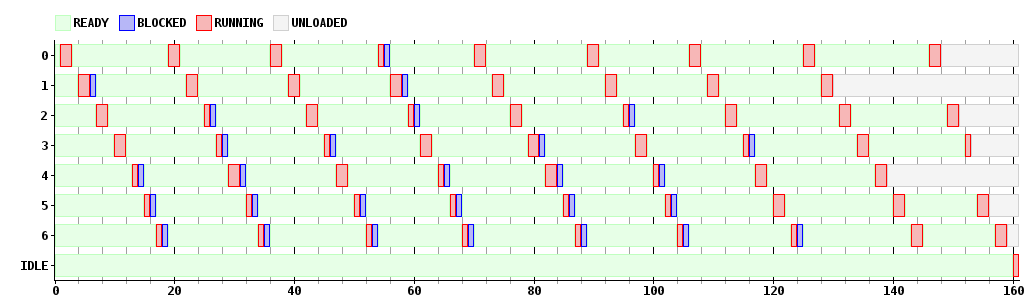
\includegraphics[width=16cm]{../simusched/outputs/ej7/rr-ej7-1-2.png}
\end {center}

\par Diagrama con 5 ciclos de quantum:
\begin {center}
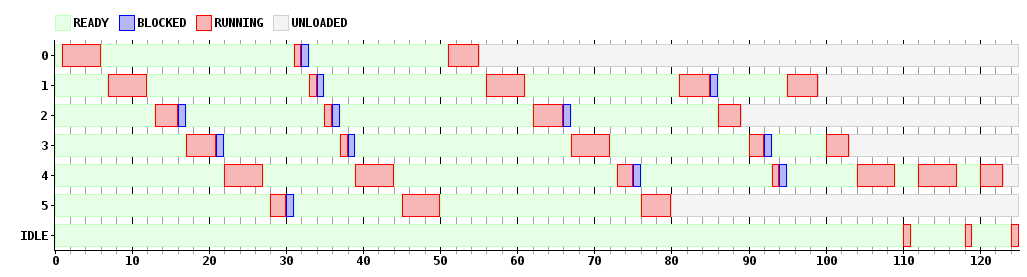
\includegraphics[width=16cm]{../simusched/outputs/ej7/rr-ej7-1-5.png}
\end {center}

\par Diagrama con 7 ciclos de quantum:
\begin {center}
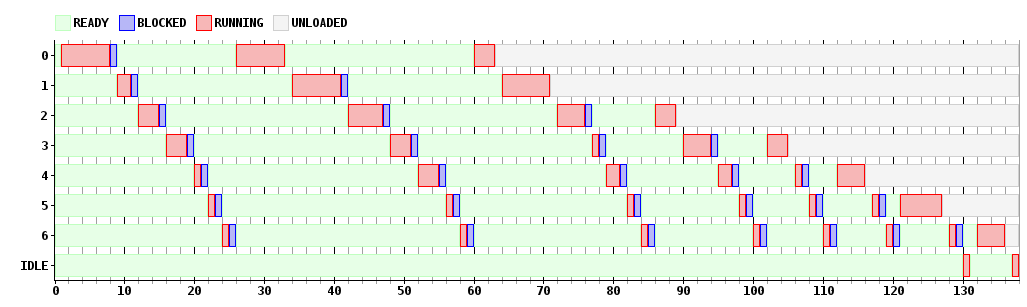
\includegraphics[width=16cm]{../simusched/outputs/ej7/rr-ej7-1-7.png}
\end {center}

\par Diagrama con 9 ciclos de quantum:
\begin {center}
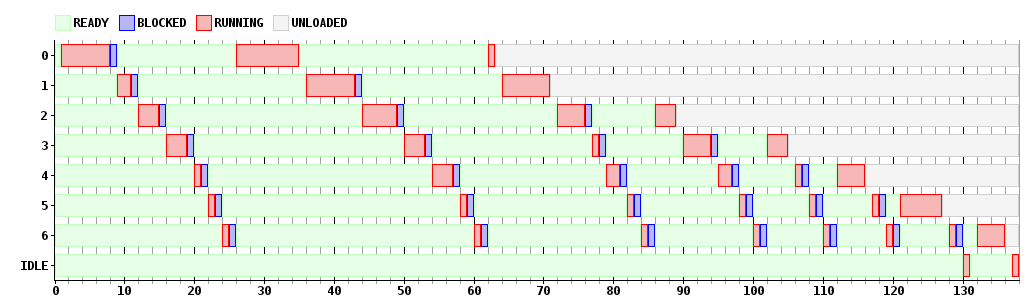
\includegraphics[width=16cm]{../simusched/outputs/ej7/rr-ej7-1-9.png}
\end {center}

\par Diagrama con 12 ciclos de quantum:
\begin {center}
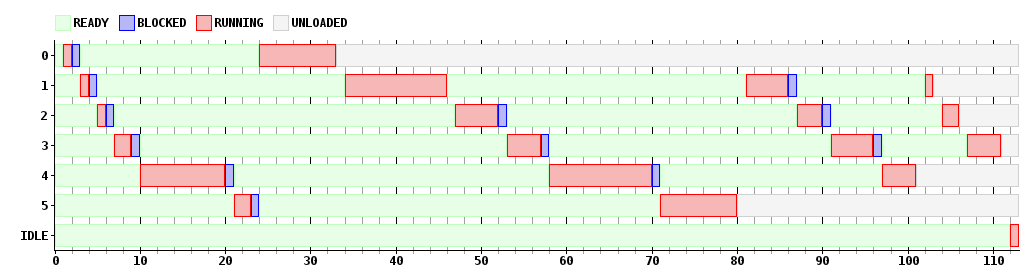
\includegraphics[width=16cm]{../simusched/outputs/ej7/rr-ej7-1-12.png}
\end {center}

\par Diagrama con 17 ciclos de quantum:
\begin {center}
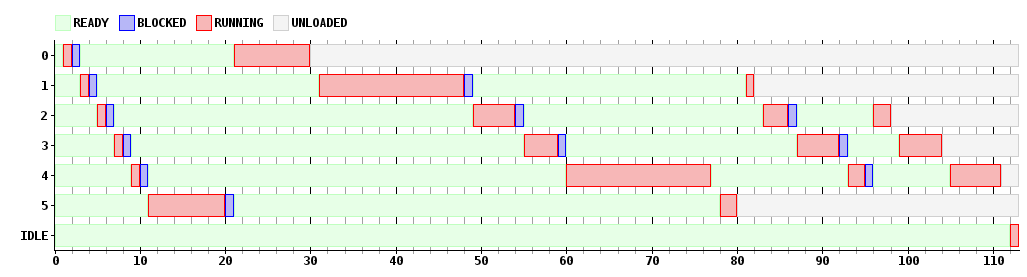
\includegraphics[width=16cm]{../simusched/outputs/ej7/rr-ej7-1-17.png}
\end {center}

\par Diagrama con 21 ciclos de quantum:
\begin {center}
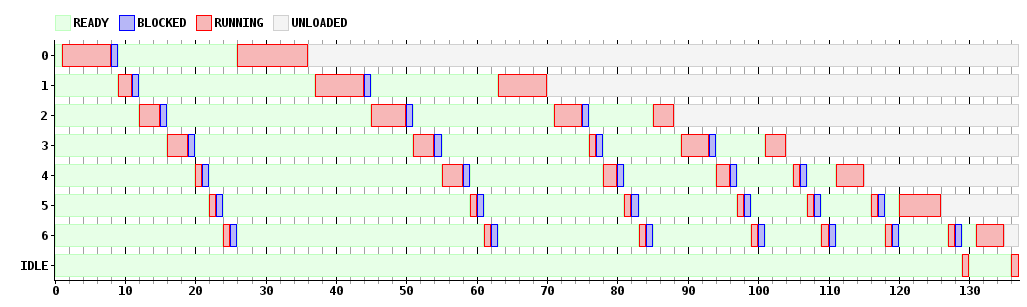
\includegraphics[width=16cm]{../simusched/outputs/ej7/rr-ej7-1-21.png}
\end {center}

Se puede observar que a medida que los ciclos del quantum aumentan, las tareas finalizan más rapido, debido a que se les da más tiempo de ejecución, hay un menor cambio de contexto entre los procesos y ocurren menos bloqueos por intervalo de ejecución del proceso.
\\
Para este lote de tareas en particular, suele ser más eficiente asignarle una cantidad grande de ciclos por quantum,  ya que se realizarán menos bloqueos y cada proceso podrá finalizar en la menor cantidad de $"$cortes$"$ de ejecución, pero no excesiva, porque, como se aprecia en las imágenes, entre 12 y 21  ciclos por quantum todos tardan lo mismo en finalizar y no mejora la eficiencia.
\\
Con un quantum de 21 ciclos, se puede notar que lo que más influye en cada proceso son los bloqueos que se producen y no tanto el corte porque no le quedan más ciclos, produciendo cambios de contexto obligatorios y empeorando bastante la optimización del Round Robin frente a otros algoritmos de scheduling.



  \newpage
\section{Ejercicio 8}
\subsection{Enunciado}

\subsection{Soluci\'on}

%SI QUIEREN AGREGAR IMAGENES COPIEN EL SIGUIENTE CODIGO
%\begin {center}
%\includegraphics[width=12cm]{./graphEj1.jpg}
% grafico.eps: 0x0 pixel, 300dpi, 0.00x0.00 cm, bb=50 50 410 302
%\end {center}

  \newpage

\end{document}
